
\section{Guiding}

\subsection{Overview}

\subsubsection{Requirements and Constraints}
The guiding system's design is driven by the need for precision, stability, and reliability in the hyperloop pod's trajectory. Key requirements include accurate track alignment, robust response to dynamic conditions, and compatibility with the pod's overall architecture. Constraints involve mostly physical dimensions, as the subsytem is decoupled from the rest of the pods development.

\subsubsection{Concept}
The guiding subsystem is conceptualized to maintain the pod's course with high precision while minimizing lateral and vertical deviations. The selection of this concept is based on its ability to enhance safety, improve ride comfort, and ensure operational efficiency. We have decided to keep this years guiding system as simple as possible as we are currently developing levitation technices which will invcorporate a more advanced guiding system in its assembly. This means, that the guiding system does not incorporate sensors, actuators, or other control algorithms. These will be added in the next iteration to continuously adjust the pod's position, aligning with the track's optimal path.

\subsubsection{Size, Components, and Appearance}
The guiding system consists of minimal parts, selected for their reliability, durability, and performance characteristics, ensuring the system's effectiveness and longevity. The table below outlines the materials, mass, dimensions, and other critical attributes of each component, providing a clear overview of the system's physical characteristics and how it integrates into the pod's design.

\begin{table}[ht]
\centering
\label{table:components}
\begin{adjustbox}{width=\textwidth,center}
\begin{tabular}{|>{\bfseries}m{2.5cm}|m{1.4cm}|m{1.7cm}|m{2.1cm}|m{2.2cm}|m{2.6cm}|m{2.2cm}|}
\hline
Component & Number & Mass [kg] & Size [mm] & Material & Manufacturing process & In-house/ Outsourced \\
\hline
Guiding Wheels & x4 & 0.3 & 35 x 30 & Al6061 T6 & Latheturning & In-house \\
Rocker Arms & x8 & 0.2 & 130 x 50 x 8 & C45 & Lasercut & In-house \\
Bearings Small& x16 & 0.1 & 20x30x50 & Steel & -&  Outsourced  \\
Bearings Large & x8 & 0.1 & 30x40x60 & Steel & -& Outsourced \\
Bearings Cylinder & x8 & 0.2 & 30x40x60 & Steel & -& Outsourced \\
Spring Dampener & x2 & 0.4 & 30x150 & Steel & -& Outsourced \\
Gas Dampemer & x2 & 0.2 & 15x150 & Steel & -& Outsourced \\

\hline
\end{tabular}
\end{adjustbox}
\caption{Components and Manufacturing Details}
\end{table}

\subsection{Theoretical Concepts}

The guiding system's design draws from classical mechanics, specifically kinematics and dynamics that govern the motion of bodies under force. The spring within the front guiding mechanism adheres to Hooke's Law, stating that the force exerted by a spring is proportional to its displacement, expressed as\\
 \( F = -kx \)\\
 This relation allows the guiding system to mitigate shocks and maintain stability.

Dynamic balance is also crucial, with the guiding system maintaining the pod's trajectory by ensuring the centripetal force (\( F_c = mv^2/r \)) counteracts any centrifugal force arising from the pod's velocity and the track's curvature. Frictional forces play a part, characterized by \( f = \mu N \), where \( f \) is the frictional force, \( \mu \) the coefficient of friction, and \( N \) the normal force.

Moreover, damping is considered to reduce oscillations, with the damping force (\( F_d = -cv \)) being velocity-dependent. These principles collectively ensure the guiding system maintains the pod's course, absorbs energy from track irregularities, and supports high-speed stability.


\subsection{Design Process and Appearance}
\subsubsection{CAD Models and Technical Drawings}
% Present CAD models and technical drawings.

\begin{figure}[!ht]
  \centering
  \begin{minipage}[b]{0.45\linewidth}
    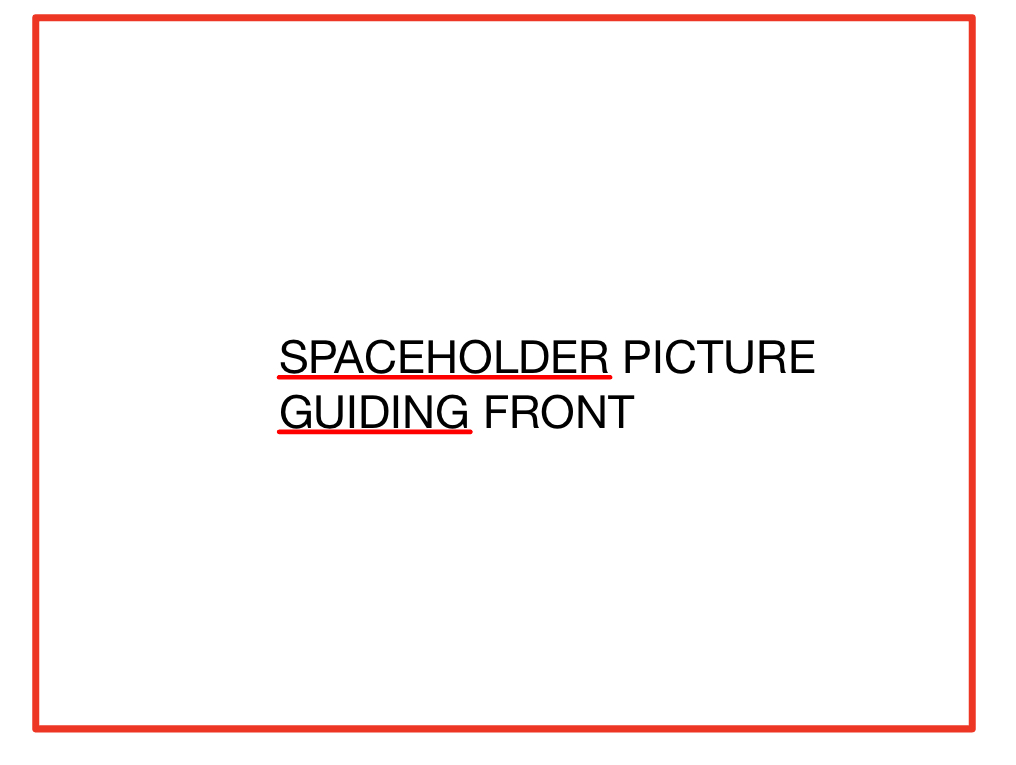
\includegraphics[width=\linewidth]{texfiles/mech/eimg/guiding/guiding_front_1.jpg}
    \caption{CAD Guiding Front}
    \label{fig:guiding_front}
  \end{minipage}
  \hspace{0.5cm}
  \begin{minipage}[b]{0.45\linewidth}
    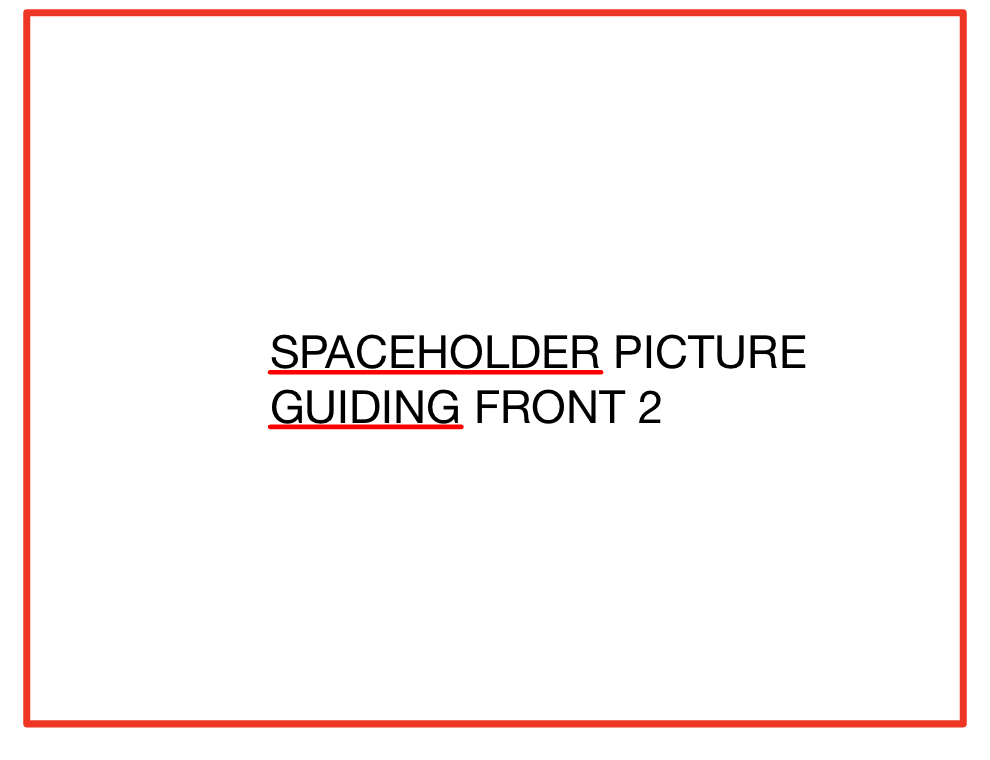
\includegraphics[width=\linewidth]{texfiles/mech/eimg/guiding/guiding_front_2.jpg}
    \caption{CAD Guiding Rear}
    \label{fig:guiding_rear}
  \end{minipage}
\end{figure}

\begin{figure}[!ht]
  \centering
  \begin{minipage}[b]{0.45\linewidth}
    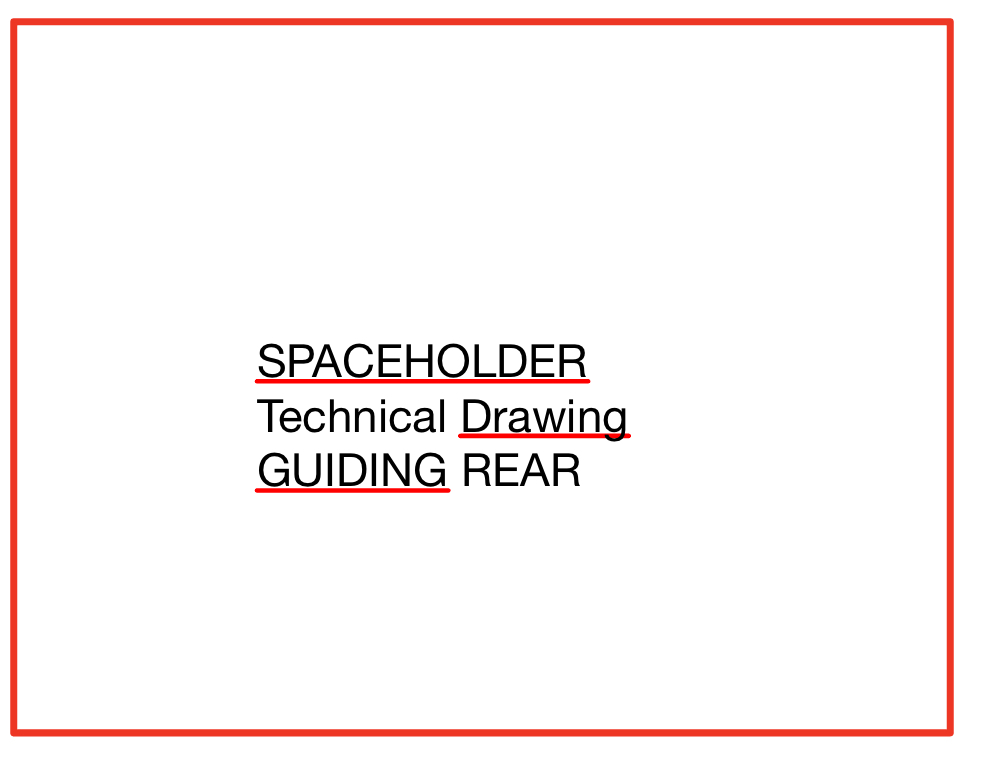
\includegraphics[width=\linewidth]{texfiles/mech/eimg/guiding/guiding_tech_rear.jpg}
    \caption{CAD Guiding Front \#2}
    \label{fig:guiding_front_2}
  \end{minipage}
  \hspace{0.5cm}
  \begin{minipage}[b]{0.45\linewidth}
    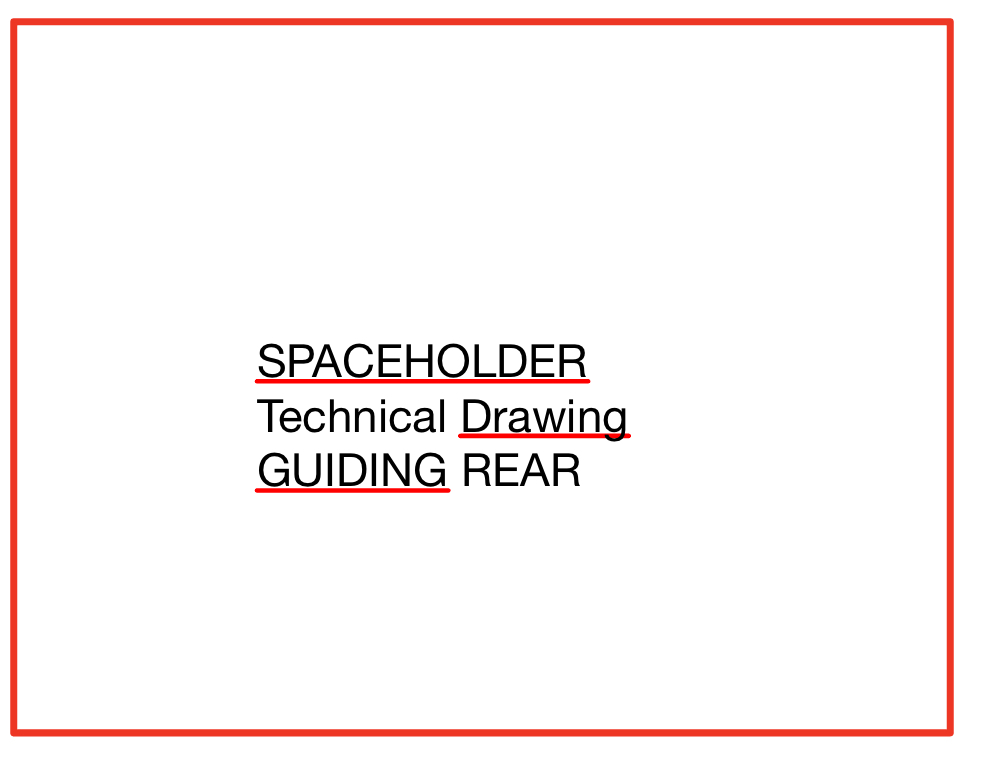
\includegraphics[width=\linewidth]{texfiles/mech/eimg/guiding/guiding_tech_rear.jpg}
    \caption{CAD Guiding Rear 2}
    \label{fig:guiding_rear_2}
  \end{minipage}
\end{figure}

\begin{figure}[!ht]
  \centering
  \begin{minipage}[b]{0.45\linewidth}
    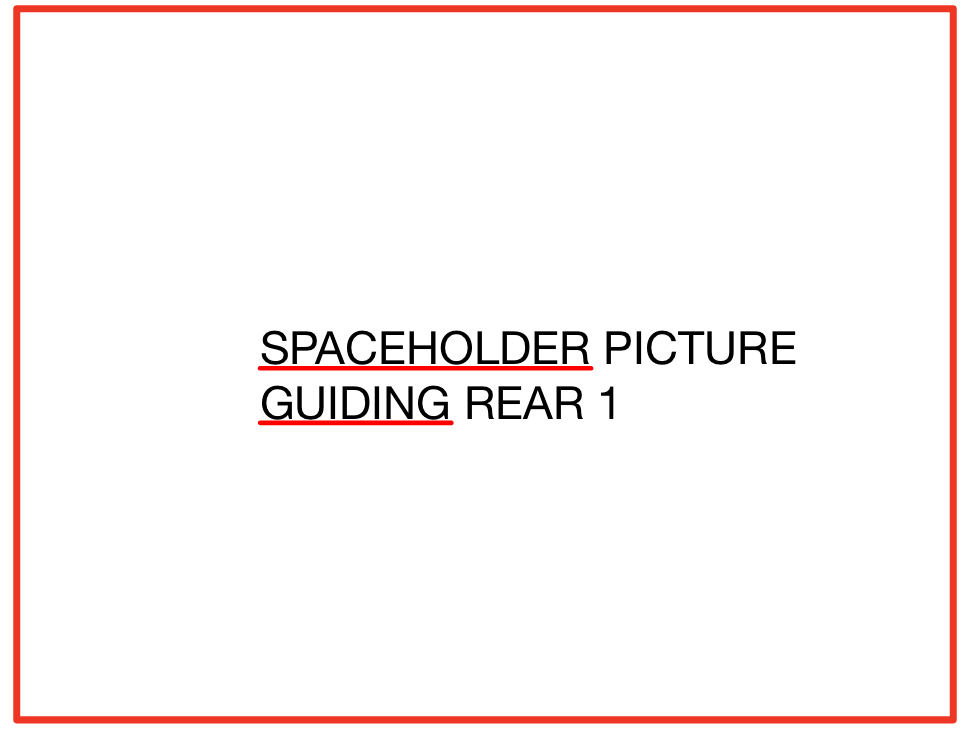
\includegraphics[width=\linewidth]{texfiles/mech/eimg/guiding/guiding_rear_1.jpg}
    \caption{Technical Drawing Guiding Front }
    \label{fig:guiding_front_2}
  \end{minipage}
  \hspace{0.5cm}
  \begin{minipage}[b]{0.45\linewidth}
    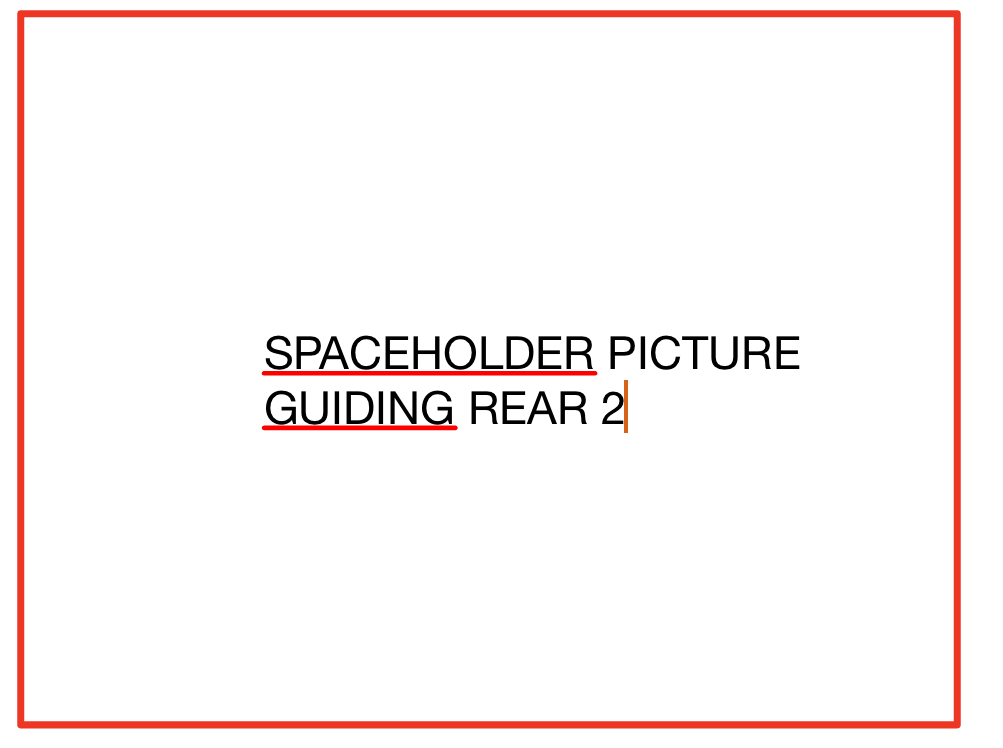
\includegraphics[width=\linewidth]{texfiles/mech/eimg/guiding/guiding_rear_2.jpg}
    \caption{Technical Drawing  Guiding Rear}
    \label{fig:guiding_rear_2}
  \end{minipage}
\end{figure}


\subsubsection{Materials}

For the guiding system, the choice of Al 6061 T6 is based on its favorable attributes that align well with the operational demands of the hyperloop. This aluminum alloy offers a commendable blend of strength, lightweight characteristics, and cost-effectiveness, making it a suitable material for high-performance applications like the hyperloop. Its durability ensures resistance to mechanical stresses, and its lightweight nature enhances the pod's overall efficiency. Moreover, the material's machinability facilitates the precision manufacturing of components. The selection of a material with lower hardness than the track surface (S365) used by SwissLoop is strategic to prevent any potential damage to the track while maintaining the guiding system's integrity. Additionally, the rocker arms are fabricated from C45 steel sheet, sourced from the same material as the braking assembly, providing sufficient strength for their function without unnecessary material diversity.

\subsubsection{Design Rationale}
\textbf{WILL BE ADDED SOON}

\subsubsection{FEM Results}
% Present FEM results for worst-case scenarios.
\textbf{WILL BE ADDED SOON}
\subsubsection{Calculations}
% Provide reasoning and necessary calculations.
\textbf{WILL BE ADDED SOON}
\subsubsection{Mesh and Boundary Conditions}
% Provide details on mesh, boundary conditions, and diagrams.
\textbf{WILL BE ADDED SOON}


\subsection{Manufacturing Process}

The manufacturing process for the front and rear guiding system is designed to be straightforward and efficient, ensuring the creation of robust and reliable components. The following steps detail the process:

\begin{enumerate}
    \item \textbf{CNC Cutting of Chassis Mounts:} Utilizing Computer Numerical Control (CNC) technology, the chassis mounts are cut with precision. This ensures they adhere to the exact dimensions required for stability and alignment.
    
    \item \textbf{Laser Cutting of Rocker Arms:} The rocker arms are produced using a laser cutter, which precisely slices through the C45 steel sheet, ensuring the arms' strength and durability.
    
    \item \textbf{Guiding Wheel Fabrication:} A lathe is employed to manufacture the guiding wheels, ensuring they are shaped accurately to meet design specifications and ensure effective operation.
    
    \item \textbf{Bearing and Spring Assembly:} Bearings are meticulously pressed into place, facilitating smooth motion and reducing friction. The springs are then mounted, providing the necessary suspension functionality to absorb impacts and maintain stability.
    
    \item \textbf{Mounting of Chassis Mounts:} The chassis mounts are affixed using bolts and an adhesive, creating a secure and enduring connection capable of withstanding the rigors of hyperloop travel.
    
    \item \textbf{Adjustment of Spring Tension:} The system includes a gewinderversteller, enabling the adjustment of spring tension. This allows for fine-tuning of the springs' pre-tension, optimizing the suspension characteristics.
\end{enumerate}


\subsection{Integration Process}

The integration process for the guiding system is meticulously planned to ensure it functions independently, without interfering with other subsystems of the hyperloop pod. The key steps of the integration process include:

\begin{enumerate}
    \item \textbf{Isolation of the Guiding System:} The guiding system is engineered as a standalone module. It possesses its own designated space and mounting points on the pod's chassis, ensuring physical separation. This design choice prevents mechanical interactions with other subsystems, such as the propulsion or braking systems.
    
    \item \textbf{Independent Mounting:} To further ensure autonomy, the guiding system is mounted onto the chassis using techniques that minimize the transmission of vibrations or forces to other subsystem parts. This method aids in isolating the system's mechanical influences, enabling it to operate without impacting the functionality of adjacent components.
   \end{enumerate}
\subsection{Safety Considerations}
When designing the guiding system, significant emphasis is placed on ensuring high safety standards. This section elaborates on the safety factors, considers worst-case scenarios, and outlines additional safety measures implemented within the system.

\begin{itemize}
    \item \textbf{Safety Factors:} All structural elements of the guiding system are designed with a safety factor greater than 2. This ensures that the system has a considerable margin of safety under normal operational conditions and unexpected stresses.
    
    \item \textbf{Worst-Case Scenarios:} We analyze potential worst-case scenarios, including system failure or unexpected interactions with the track. For each scenario, we have developed contingency plans to mitigate risks, ensuring the system's integrity and the safety of the pod.
    
    \item \textbf{Isolation and Non-interference:} The guiding system is designed to operate independently, minimizing the risk of interference with other subsystems. This isolation enhances the overall safety of the pod by reducing the complexity of interactions between different components.
    


\end{itemize}

By adhering to these safety considerations, the guiding system is designed to operate reliably, prioritizing the safety of the pod.



\subsection{FMEA Results Discussion}
% Detail FMEA, risk assessments, and mitigation measures.

\subsection{Testing}

This testing plan outlines the procedures for ensuring the integrity and functionality of the guiding system components and assembly.
\paragraph{Component Inspection}
\begin{itemize}
    \item \textbf{Objective:} Ensure each component is free from cracks and other potential integrity issues.
    \item \textbf{Method:} Perform visual inspections and non-destructive testing (e.g.  dye penetrant testing) to detect any flaws.
\end{itemize}

\paragraph{Assembly Check for free movemend}
\begin{itemize}
    \item \textbf{Objective:} Verify smooth operation under maximum compression without obstruction.
    \item \textbf{Method:} Simulate maximum compression on the assembled system and monitor for unrestricted movement and alignment.
\end{itemize}

\paragraph{Stress Test on Chassis Mounts}
\begin{itemize}
    \item \textbf{Objective:} Confirm the chassis mounts can endure operational stresses without failure.
    \item \textbf{Method:} Apply static loads that replicate or exceed operational stresses, using appropriate sensors to measure response.
\end{itemize}
